The previous section presented the likelihood $p(x | z)$, which describes the generation of an image $x$ given a catalog $z$, as well as a prior distribution $p(z)$ over the space of all catalogs. 
The central quantity in Bayesian statistics is the posterior distribution $p(z|x)$, which captures the likelihood of a certain catalog $z$ given 
an observed image $x$. 

% \jeff{Better to just say something about the posterior being the quantity of interest, rather than doing this question thing.}
However, in most
nontrivial probabilistic models, including ours, the posterior distribution is intractable to calculate.
%\jeff{It's more like certain functionals of the posterior distribution we're after; e.g., the mean and some measures of uncertainty. 
%Perhaps we just want to say here that ``A central quantity in Bayesian statistics is the posterior distribution'', rather that saying what we ``seek''.  My concern is that astronomy reviewers will say that the posterior isn't what matters for scientific inference....it's population-level quantities or something like that. We need to address that concern in the introduction and the discussion section, but it'd be better to avoid having this discussion in the VI section.
%}
% However, in most nontrivial probabilistic models, including ours, the posterior distribution is intractable.
% \jeff{Can you say ``computing the posterior distribution exactly is intractable'' here instead?
% An ``exact posterior distribution'' isn't really a thing. Only ``posterior distribution'' is defined.
% }

Variational inference~\cite{Blei_2017_vi_review, Jordan_intro_vi, Wainwrite_graph_models_vi}
posits a family of distributions $\mathcal{Q}$ and seeks
the distribution $q^*\in \mathcal{Q}$ that is closest to the posterior
in $\KL$ divergence. Suppose the family of distributions $\mathcal{Q}$ is parameterized by a real-valued vector $\eta$. We seek the optimal $\eta^*$ 
satisfying
\begin{align}
   \eta^* &= \argmin_{\eta} \mathrm{KL}\Big[\,q_\eta(z | x)\, \| \,p(z | x )\,\Big].
   \label{eq:kl_objective}
\end{align}

Minimizing the $\KL$ divergence is equivalent to maximizing the ELBO (evidence lower bound), defined as 
\begin{align}
    \mathcal{L} = 
    \Expect_{q_\eta(z | x)}\Big[\log p(x, z) - \log q_\eta(z | x)\Big].
    \label{eq:elbo}
\end{align}
Computing the ELBO does not require computing the marginal distribution $p(x)$, which is intractable, nor does it
require computing the posterior distribution $p(z | x)$.

\subsection{The variational distribution}
\label{sec:var_distr}
% We now describe our family of distributions $\mathcal{Q}$. 
Traditionally in variational inference, the posterior approximation 
$q_\eta$ depends on data $x$ implicitly, 
in that $\eta^*$ is chosen according to~\eqref{eq:kl_objective}. In this case, $q_\eta(z | x)$ is usually written $q_\eta(z)$. For a new observation $\tilde x$, the optimization problem~\eqref{eq:kl_objective} must be solved again for $\tilde x$ to find an 
approximation to the posterior $p(z | \tilde x)$. 

In {\itshape amortized} variational
inference~\cite{kingma2013autoencoding, rezende2014stochastic}, $q_\eta$ explicitly depends on data $x$. A flexible, parameterized function, typically a neural network, maps input data $x$ to
a distribution on $z$. 
The variational parameters $\eta$ in~\eqref{eq:kl_objective} 
are the neural network weights. 
After the neural network is trained using 
objective~\eqref{eq:kl_objective}, the 
approximate posterior $q_\eta(z | \tilde x)$ for a new data point 
$\tilde x$ can be evaluated with a single forward pass through the neural network. 
Re-optimization is not needed for every new data point $\tilde x$. 
\bryan{mention NN also good for nonconvex optimization?}
% \jeff{A reader probably won't understand what you mean by  ``an amortized approach'' here.}

In the ensuing subsections, we detail the construction of our variational distribution. 
% \jeff{You probably want to cite Kingma and Welling 2014 somewhere around here}

\subsubsection{The factorization}
\label{sec:factorization}
To make the objective in \eqref{eq:kl_objective} tractable in most 
applications, the family $\mathcal{Q}$ is restricted to probability distributions 
that limit conditional dependencies between latent variables. In the most extreme case, called mean-field variational inference, the variational distribution factorizes across all latent variables. 

Our factorization has a spatial structure. We decompose the full $H \times W$ image into disjoint $R \times R$ tiles that cover the image. Each tile $\tilde x_{st}$ is composed of pixels:
\begin{align}
    \tilde x_{st} = \{x_{hw} : Rs \leq h \leq R(s+1) \text{ and } Rt \leq w \leq R(t+1)\}.
    \label{eq:tiles}
\end{align}
Let $S = \frac{H}{R}$ and $T = \frac{W}{R}$ and assume that $H$ and $W$ are multiples of $R$. The tiles cover the image, so $s$ and $t$ range over $s = 1, ..., S$ and $t = 1, ..., T$. See Figure~\ref{fig:ex_tiles} for a schematic.
% \jeff{Also, we should define what tiles are.}
% \jeff{The dimension of the tiles maybe better in uppercase: the other ``structural constants'' are uppercase (e.g., $H$, $W$).}
\begin{figure}[!ht]
    \centering
    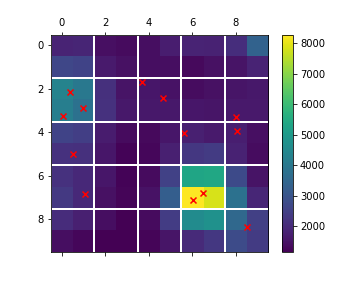
\includegraphics[width = 0.5\textwidth]{figures/example_tiled.png}
    \vspace{-1cm}
    \caption{Tiling a 10 x 10 image into 2 x 2 tiles.}
    \label{fig:ex_tiles}
\end{figure}
% \jeff{Would you want to introduce a term like ``padded tiles'' somewhere to refer to the tile plus some of the nearby pixels around it? Tiles are disjoint from each other but padded tiles overlap some with each other.}

Let $\tilde N^{(s, t)}$ be the number of stars in tile 
$(s,t)$. 
For the locations and fluxes, we construct a {\itshape triangular array}  of latent variables on each tile:
\begin{align}
    \tilde\ell^{(s, t)} &= (\tilde\ell_{N, i}^{(s, t)} : i = 1, ..., N; N = 1, 2, ...); \\
    \tilde f^{(s, t)} &= (\tilde f_{N, i}^{(s, t)} : i = 1, ..., N; N = 1, 2, ...),
\end{align}
where $\tilde\ell_{N, i}^{(s, t)}$ and $\tilde f_{N, i}^{(s, t)}$ are the elements of the triangular array corresponding to location and fluxes, respectively. 
% \jeff{Where is $\tilde\ell_{N, i}^{(s, t)}$ defined?
% }

While locations on the full image are parameterized to be
$\ell_i \in [0, H]\times[0, W]$, locations on tiles are parameterized to be $\tilde\ell_{N, i}^{(s, t)} \in [0, R]\times[0, R]$. The fluxes $\tilde f_{N, i}^{(s, t)}$ are vectors (one flux for each band) in $\mathbb{R}^B$ where each entry is positive. 

We call $(\tilde N^{(s, t)}, \tilde \ell^{(s, t)}, \tilde f^{(s, t)})_{s=1,t=1}^{S,T}$ the {\itshape tile latent variables}; 
succinctly, denote tile latent variables as $\tilde z$. 
We will define a distribution on $\tilde z$. 
We also construct a mapping from $\tilde z$ to 
the catalog $z = \{N, (\ell_i, f_{i,1}, ..., f_{i,B})_{i = 1}^N\}$. Thus, a distribution 
on the tile latent variables $\tilde z$ induces 
a distribution on our latent variable of interest, the catalog $z$. 

We detail the mapping $\tilde z\mapsto z$. 
The number of stars in the catalog is 
\begin{align}
    N = \sum_{s=1}^{S}\sum_{t=1}^T \tilde N^{(s, t)}. 
\end{align}
For every tile $(s,t)$ we index into the $\tilde N^{(s,t)}$-th
row of the triangular array of locations and fluxes. 
The fluxes in the catalog are
\begin{align}
    \{f_i\}_{i=1}^N = \Big\{\tilde f_{\tilde N^{(s, t)}, i}^{(s, t)} : i = 1, ..., \tilde N^{(s, t)}, s = 1, ..., S, t = 1, ..., T \Big\}.
\end{align}
The corresponding locations in the catalog are
\begin{align}
    \{\ell_i\}_{i = 1}^N = \Big\{\tilde \ell_{N^{(s, t)}, i}^{(s, t)} + 
    \begin{pmatrix}
    Rs \\ Rt
    \end{pmatrix} 
    : i = 1, ..., N^{(s, t)}, s = 1, ..., S, t = 1, ..., T\Big\}.
\end{align}
where we took the stellar location within the tile and shifted it by the location of the tile $(Rs, Rt)$. 

We have defined a mapping from tile latent variables to the catalog of interest, 
\begin{align}
 \big(\tilde N^{(s, t)}, \tilde \ell^{(s, t)}, \tilde f^{(s, t)}\big)_{s=1, t = 1}^{S, T}
\mapsto     
\{N, (\ell_i, f_{i,1}, ..., f_{i,B})_{i = 1}^N\}.
\label{eq:patch_to_full_map}
\end{align}
Therefore, a distribution on the tile latent variables induces a distribution on catalogs. 

Our distribution on $\tilde z$ factorizes over image tiles:
\begin{align}
    \tilde q_\eta\big( \big(\tilde N^{(s, t)}, \tilde \ell^{(s, t)}, \tilde f^{(s, t)}\big)_{s=1, t = 1}^{S, T}|x\big) 
    &=
    \prod_{s = 1}^S \prod_{t=1}^T
    \tilde q_\eta\big(\tilde N^{(s, t)}, \tilde \ell^{(s, t)}, \tilde f^{(s, t)} | x\big).
    \label{eq:factorize_patches}
\end{align}
Within each tile $(s,t)$, the distribution also fully factorizes: 
\begin{align}
    \tilde q_\eta\big(\tilde N^{(s, t)}, \tilde \ell^{(s, t)}, \tilde f^{(s, t)} | x\big)
    &= 
    \tilde q_\eta\big(\tilde N^{(s, t)} | x\big)
    \prod_{n = 1}^\infty \prod_{i = 1}^n 
    \tilde q_\eta\big(\tilde \ell_{n,i}^{(s, t)} | x\big)
    \tilde q_\eta\big(\tilde f_{n,i}^{(s, t)} | x\big).
    \label{eq:factorize_within_patch}
\end{align}

If $\tau$ is the mapping in~\eqref{eq:patch_to_full_map}, then the variational distribution on catalogs $z$ is
\begin{align}
    q_\eta(z | x) := \tilde q_\eta(\tau^{-1}(z) | x),
    \label{eq:pull_back_of_q}
\end{align}
where $\tau^{-1}(z)$ is the pre-image of $z$.

\noindent{\bf Evaluating the variational distribution}

% \noindent We can use the mapping~\eqref{eq:patch_to_full_map}
% to sample catalogs from our variational distribution.
% If $\tau$ is the mapping in~\eqref{eq:patch_to_full_map}, then 
% we can express the variational distribution
% on the full image catalog $z$ as 
% \begin{align}
%     z &\stackrel{d}{=} \tau\Big( \big(\tilde N^{(s, t)}, \tilde \ell^{(s, t)}, \tilde f^{(s, t)}\big)_{s=1, t = 1}^{S,T}\Big), \notag \\  
%         &\text{where } 
%         \big(\tilde N^{(s, t)}, \tilde \ell^{(s, t)}, \tilde f^{(s, t)}\big)_{s=1, t = 1}^{S,T}
%         \sim 
%         q_\eta\big( \cdot |x\big).
% \end{align}

\noindent To evaluate
the ELBO in~\eqref{eq:elbo}, 
we need to compute the probability of 
$q_\eta(z | x)$
for any given catalog $z = \{N, (\ell_i, f_{i,1}, ..., f_{i,B})_{i = 1}^N\}$. By~\eqref{eq:pull_back_of_q}, 
we need to evaluate $\tilde q_\eta(\tau^{-1}(z) | x)$. 

We remark that $\tau^{-1}(z)$ is a {\itshape set} of tile latent variables because the mapping from tile latent variables to catalogs $z$ is not injective. We detail this below. 

Locations in the catalog $\{\ell_i\}_{i=1}^N$
determine the number of stars on tile $(s,t)$. 
The number of stars $\tilde N^{(s,t)}$ is simply the count of the locations that reside within that tile:
\jeff{What does it mean to ``fall within a tile''?}
\bryan{Is reside better?}
\begin{align}
\tilde N^{(s,t)} = \sum_{i=1}^N 
\mathbf 1 \Big\{\ell_i\in [Rs, R(s+1)] \times [Rt, R(t+1)]\Big\},
\end{align}
where $\mathbb{I}\{\cdot\}$ is the indicator function, equal to one if true and zero if false.
% \jeff{I more often see $\mathbf 1$ used as the indicator function}

Now we consider $\tilde\ell^{(s, t)}$ and $\tilde f^{(s, t)}$, the triangular array of locations and fluxes on tile $(s,t)$. 
For each $(s,t)$, the $\tilde N^{(s,t)}$-th row 
of the triangular array of fluxes and locations are 
determined by the locations and fluxes of stars that landed in tile $(s,t)$. However, the other rows 
of the triangular arrays are not determined by 
the catalog $z$, and are free to take any value in their domain. Therefore, the mapping $\tau$ is not injective. 

To evaluate the probability of $\tau^{-1}(z)$ under $\tilde q_\eta$, we must marginalize over the rows of the triangular arrays $\ell^{(s, t)}$ and $\tilde f^{(s, t)}$ that are not determined by $z$. However, 
because $\tilde q_\eta$ fully factorizes, the terms 
in~\eqref{eq:factorize_within_patch} where $n \not= \tilde N^{(s,t)}$ do not enter the
% \jeff{What does ``drop out'' mean?}
product
after marginalization.
Applying this observation and combining~\eqref{eq:factorize_within_patch} and ~\eqref{eq:factorize_patches}, we obtain that
\begin{align}
    \tilde q(\tau^{-1}(z) | x) = \prod_{s=1}^S\prod_{t=1}^T
    \Big\{
    \tilde q_\eta(\tilde N^{(s,t)} | x) 
    \prod_{i = 1}^{\tilde N^{(s,t)}}
    \tilde q_\eta\big(\tilde \ell_{\tilde N^{(s,t)},i}^{(s, t)} | x\big)
    \tilde q_\eta\big(\tilde f_{\tilde N^{(s,t)},i}^{(s, t)} | x\big)
    \Big\}.
\end{align}
In other words, given a catalog $z$,
we convert $z$ to tile random variables;
to compute $q_\eta(z | x)$, it suffices to evaluate $\tilde q_\eta$ only at the rows of triangular 
arrays determined by the number 
of stars falling in each tile. 


% There is a bijection between latent variables on each tile and latent variables on the full image (locations on the full image map to locations on image tiles and vice-versa). 
% \jeff{It's not clear what it means for a latent variable to be ``on a tile''. Why a bijection? They're the same latent variables, right?}
% Thus, a variational distribution for latent variables on tiles induces a variational distribution for latent variables on the full image.
% \jeff{This isn't such a good way to explain it. Better to directly explain the variational distribution over the whole image, from top down, introducing the concept of tiles along the way. Perhaps at the end make the point that our choice of variational distribution does not render the problem embarrassingly parallel.}
% If $\tau$ is the mapping in~\eqref{eq:patch_to_full_map}, then 
% we can express the variational distribution
% on the full image catalog as 
% \begin{align}
%     z &\stackrel{d}{=} \tau\Big( \big(\tilde N^{(s, t)}, \tilde \ell^{(s, t)}, \tilde f^{(s, t)}\big)_{r=1, t = 1}^{s, t}\Big), \notag \\  
%         &\text{where } 
%         \big(\tilde N^{(s, t)}, \tilde \ell^{(s, t)}, \tilde f^{(s, t)}\big)_{r=1, t = 1}^{s, t}
%         \sim 
%         \prod_{r = 1}^R \prod_{t=1}^T q_\eta\big(\tilde N^{(s, t)}, \tilde \ell^{(s, t)}, \tilde f^{(s, t)} | x\big).
% \end{align}
% \jeff{I suggest getting rid of $T$ here. This bijection is a confusing way to explain things. Instead, to refer to the pixels in tile (i, j), you might define
% \[
%     \tilde x_{i,j} = \{x_{hw} : Si \ge h > S(i + 1) \text{ and } Sj \ge w > S(j+1)\}.
% \]
% You could do the same thing for $\tilde f$, etc.
% }
% \jeff{Is there somewhere you say that in the variational distribution, $N = \sum_{k=1}^K N^{(k)}$ ? That might be a good way to put it.}

\subsubsection{Distributions on image tiles}
We describe the distribution on each tile,
$\tilde q_\eta\big(\tilde N^{(s, t)}, \tilde \ell^{(s, t)}, \tilde f^{(s, t)} | x\big)$. Dropping the index 
$(s,t)$ in this subsection, 
\begin{align}
    \tilde N &\sim \text{Categorical}(
    \omega; 0, ..., N_{max});  \label{eq:var_distr_n}\\
	\tilde \ell_{\tilde N, i} / R &\sim \text{LogitNormal}(\mu_{\ell_{\tilde N, i}}, \text{diag}(\nu_{\ell_{\tilde N, i}}) )\label{eq:var_distr_loc}; \\
	\tilde f^b_{\tilde N, i} &\sim \text{LogNormal}(\mu_{f^b_{\tilde N, i}}, \sigma^2_{f^b_{\tilde N, i}}), \label{eq:var_distr_f}
\end{align}
\jeff{I suggest writing the parameters of these distributions as functions of the padded tile. For example, I'd write
\[
    \tilde N_{rt} \sim \text{Categorical}\left(h_\eta(\tilde{x}_{rt})\right).
\]
Here $h_\eta$ is a neural network. ($\eta$ are variational parameters).
I didn't drop the $rt$ subscript above because I wanted to make the point that the same $h_\eta$ is applied to all tiles.
}
\bryan{
I like this idea. I can introduce {\itshape padded} tiles,  
\[
\hat x^{(s,t)} = 
    \{x_{hw} : R(s+1) + P \geq h > Rs - P \text{ and } 
    R(t+1) + P\geq w > Rt - P\}.
\]
That is, we took the tiles from~\eqref{eq:tiles}
and padded each tile with $P$ pixels. Note
that tiles are disjoint, while padded tiles are not. 

I want to say that a neural network 
$h_\eta(\hat x^{(r,s)})$ that maps 
to a common concatenated vector of 
parameters describing the distributions. 

We index into this giant vector to get individual distributional parameters. 
I'm not sure how quite to denote this though ... for example to get the mean 
parameter for the $(N,i)$-th location, we'd have $\mu_{\ell_{N, i}}(h_\eta(\hat x^{(r,t)}))$, which seems like too many indices.
This is the problem with this section in general tbh ... more work will be needed on my part to figure out how to describe this. 
}
\jeff{I see your point, the notation is tricky. The main issue with $\mu_{\ell_{N, i}}(h_\eta(\hat x^{(r,t)}))$ is the double subscript. Also, it's not great have $\ell$ as a subscript of $\mu$ because $\ell$ is a random variable.
}
\jeff{
Maybe  $\left[g_\eta(\tilde x_{rt})\right]_{N,i}$ could denote the location mean and variance for the $(N,i)$-th location?
And $\left[h_\eta(\tilde x_{rt})\right]_{N,i}$ could denote the flux mean and variation?
}
for $i = 1, ..., \tilde N$; $\tilde N = 1, ..., N_{max}$. The latent variables also fully factorize within each tile. Note that in the exact posterior, $\tilde N$ has support on the nonnegative integers; in the variational distribution, we truncate at some large $N_{max}$. 
% \jeff{Do we? I thought it was just the variational distribution that doesn't have support past $N_{max}$. The posterior has support over all natural numbers.}


These distributions were taken for convenience: fluxes are positive and right skewed, so we place a normal distribution on log-fluxes; locations are between zero and $R$, so 
we place a normal distribution on the logit of the location scaled by $1 / R$. 

\subsubsection{Neural network architecture}
\label{sec:nn_archetecture}
On each tile, the distributional parameters 
in \eqref{eq:var_distr_n}-\eqref{eq:var_distr_f} are the output of a neural network.
\jeff{The parameters of the variational distribution are the weights of the neural network, not the outputs.}
\bryan{How do you recommend that I call the 
parameters in \eqref{eq:var_distr_n}-\eqref{eq:var_distr_f}?
The $\omega$, $\mu$'s, etc?}
\jeff{See comment above.}
The input to the neural network is a $S \times S$ tile, padded with surrounding pixels.
For cataloging the crowded starfield M2 (Section~\ref{sec:m2_results}),
we set $S = 2$ and padded the tile with three pixels.
\jeff{You may need to explain what padding is; e.g., what did you pad it with?}
% For our test on a sparse field (Section~\ref{sec:sparse_field}), we set $S = 50$ with no padding. 

Let $\hat x^{(s,t)}$ denote the padded tile (which includes all $B$ bands) and $h_\eta$ be the neural network, which returns the collection of distributional parameters
\begin{align}
    h_\eta(\hat x^{(s,t)}) = (\omega^{(s,t)}, \mu_\ell^{(s,t)}, \nu_{\ell}^{(s,t)}, \mu_f^{(s,t)}, \sigma^{(s,t)}_f).
    \label{eq:nn_output}
\end{align}
The same neural network is evaluated for all tiles $(s,t)$. Our variational parameters are neural network weights, here denoted $\eta$. 
The architecture consisting of several convolutional layers followed by a series of fully connected layers (Figure~\ref{fig:starnet_arch}). Convolutional layers are useful for localizing stars as they make the network invariant to shifts in stellar location. The convolutional kernel in the first layer is $3\times3$ pixels, roughly the full width at half maximum (FWHM) of the PSF. The optimization of the architecture is left for future work; our primary contribution in this paper is the application of neural networks to provide a variational posterior for cataloging starfields, not the network archetecture per se. 

\begin{figure}[!tb]
    \centering
    % 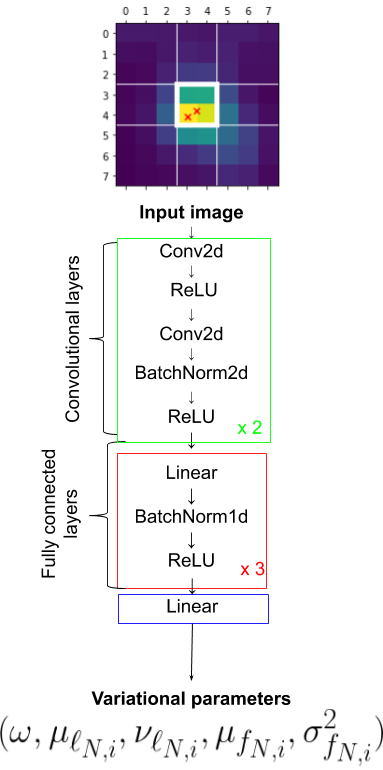
\includegraphics[width=0.4\textwidth]{figures/starnet_archetecture2.png}
    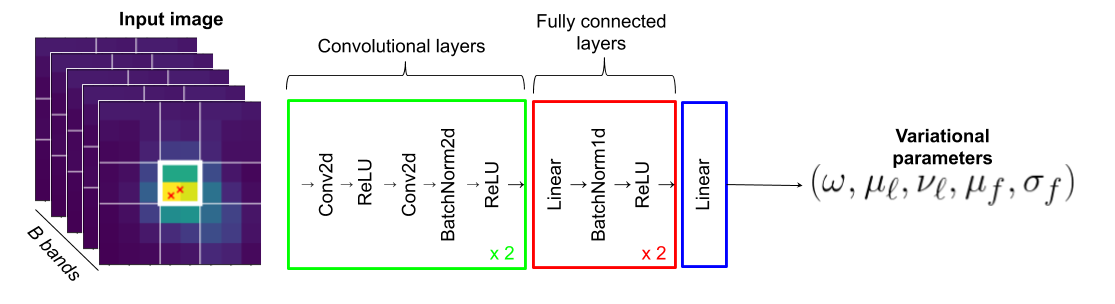
\includegraphics[width=\textwidth]{figures/starnet_archetecture3.png}
    \vspace{-0.5cm}
    \caption{The neural network returning parameters for the variational distribution on each 2 x 2 image tile. For cataloging M2, the input image is an $8\times 8$ padded tile, and the network is responsible for returning variational parameters for the cetner $2\times 2$ tile. }
    \label{fig:starnet_arch}
\end{figure}

Note the output dimension of the neural network. For each tile $(s,t)$, the categorical parameter $\omega^{(s,t)}$
lies on the simplex and has dimension $N_{max} + 1$. 
For $i = 1, ..., \tilde N$ and $\tilde N = 1, ..., N_{max}$, the location has a mean and variance on each coordinate, and the flux has a mean and variance for each band. Thus, for star indexed by $(\tilde N, i)$, 
there are $2 \times (B + 2)$ parameters for its variational distribution. In total, the neural network has output dimension $(N_{max} + 1) + (B + 2) \times (N_{max}^2 + N_{max})$. 

% Recall that locations on the 
% full image $\ell_{N, i}$ are parameterized to be in $[0, H] \times [0, W]$. 
% On the tiles, locations $\ell^{(k)}_{N, i}$ are parameterized to be in
% $[0, s] \times [0, s]$. 

% \jeff{What does it mean to decompose an inference problem from full images into tiles?}
Thus, factorizing the variational distribution spatially controls the output dimension of the neural network. On a crowded starfield with $H = W = 100$, the number of imaged stars is on the order of $10^3$. If the neural network were to return a variational distribution on the full $100\times 100$ image, the output dimension would be on the order of $10^6$. 
On the $2\times 2$ tile, we set $N_{max} = 3$, and the output dimension of the neural network with two bands is 53. 

We emphasize that while the variational distribution factorizes over $2 \times 2$ tiles, our method does not break the inference problem on the full image into embarrassingly parallel subproblems. The evaluation of the likelihood (example, when computing the ELBO in~\eqref{eq:elbo}) is always on the full image. Light from a star within a 2 x 2 tile spills over into neighboring tiles, so the likelihood does not decouple across image tiles. 
